\documentclass[a4paper,12pt,twoside]{../includes/ThesisStyle}
\usepackage[utf8]{inputenc}
\usepackage[T1]{fontenc}

\usepackage[left=1.5in,right=1.3in,top=1.1in,bottom=1.1in,includefoot,includehead,headheight=13.6pt]{geometry}\renewcommand{\baselinestretch}{1.05}


% =============================================================================
%\usepackage[sectionbib]{chapterbib}	% Cross-reference package (Natural BiB)
%\usepackage{bibunits}
%\usepackage{natbib}					% Put References at the end of each chapter
\usepackage{algorithm}
\usepackage{alltt}
\usepackage{amsfonts}
\usepackage{amsmath}
\usepackage{amssymb}
\usepackage{cite}
\usepackage{color}
\usepackage{enumerate}
\usepackage{booktabs} % used for \midrule
\usepackage{fancyhdr}					% Fancy Header and Footer
\usepackage{graphicx}
\usepackage{ifthen}
\usepackage{latexsym}
\usepackage{multirow}
\usepackage{rotating}					% Sideways of figures & tables
\usepackage{stmaryrd}
\usepackage{subfigure}
\usepackage{url}         
\usepackage{xspace}
\usepackage[normalem]{ulem} % for \sout
\usepackage{xcolor}
\usepackage{tablefootnote}
\usepackage{pifont}

% =============================================================================

% Table of contents for each chapter
\usepackage[nottoc, notlof, notlot]{tocbibind}
\usepackage{minitoc}
\setcounter{minitocdepth}{1}
\mtcindent=15pt

\setcounter{secnumdepth}{3}
\setcounter{tocdepth}{2}
  
% =============================================================================
% Fancy Header Style Options

\pagestyle{fancy}                       % Sets fancy header and footer
\fancyfoot{}                            % Delete current footer settings

%\renewcommand{\chaptermark}[1]{         % Lower Case Chapter marker style
%  \markboth{\chaptername\ \thechapter.\ #1}}{}} %

%\renewcommand{\sectionmark}[1]{         % Lower case Section marker style
%  \markright{\thesection.\ #1}}         %

\fancyhead[LE,RO]{\bfseries\thepage}    % Page number (boldface) in left on even
% pages and right on odd pages
\fancyhead[RE]{\bfseries\nouppercase{\leftmark}}      % Chapter in the right on even pages
\fancyhead[LO]{\bfseries\nouppercase{\rightmark}}     % Section in the left on odd pages

\let\headruleORIG\headrule
\renewcommand{\headrule}{\color{black} \headruleORIG}
\renewcommand{\headrulewidth}{1.0pt}
\usepackage{colortbl}
\arrayrulecolor{black}

\fancypagestyle{plain}{
  \fancyhead{}
  \fancyfoot{}
  \renewcommand{\headrulewidth}{0pt}
}


% =============================================================================
% Clear Header Style on the Last Empty Odd pages
\makeatletter

\def\cleardoublepage{\clearpage\if@twoside \ifodd\c@page\else%
  \hbox{}%
  \thispagestyle{empty}%              % Empty header styles
  \newpage%
  \if@twocolumn\hbox{}\newpage\fi\fi\fi}

\makeatother

\newenvironment{maxime}[1]
{
\vspace*{0cm}
\hfill
\begin{minipage}{0.5\textwidth}%
%\rule[0.5ex]{\textwidth}{0.1mm}\\%
\hrulefill $\:$ {\bf #1}\\
%\vspace*{-0.25cm}
\it 
}%
{%

\hrulefill
\vspace*{0.5cm}%
\end{minipage}
}

\let\minitocORIG\minitoc
\renewcommand{\minitoc}{\minitocORIG \vspace{1.5em}}


\renewcommand{\epsilon}{\varepsilon}

% centered page environment
\newenvironment{vcenterpage}
	{\newpage\vspace*{\fill}\thispagestyle{empty}\renewcommand{\headrulewidth}{0pt}}
	{\vspace*{\fill}}
	

%=============================================================================

\usepackage{needspace}
\newcommand{\needlines}[1]{\Needspace{#1\baselineskip}}

\usepackage{xcolor}
\definecolor{source}{gray}{0.95}
% source code formatting
\usepackage{listings}
    % global settings for source code listing package
\lstset{
    basicstyle=\ttfamily\small,
    showspaces=false,
    showstringspaces=false,
    captionpos=b, 
    columns=fullflexible}

\lstdefinelanguage{ST}{
    keywordsprefix=\#,
    morekeywords=[0]{true,false,nil},
    morekeywords=[1]{self,super,thisContext},
    morekeywords=[2]{ifTrue:,ifFalse:,whileTrue:,whileFalse:,and:,or:,xor:,not:,by:,timesRepeat:},
    sensitive=true,
    morecomment=[s]{"}{"},
    morestring=[d]',
    escapechar={!},
    alsoletter={., :, -, =, +, <},
    moredelim=**[is][\itshape]{/+}{+/},
    literate=
        {^}{{$\uparrow$}}1
        {:=}{{$\leftarrow$}}1
        {~}{{$\sim$}}1
        {-}{{\sf -\hspace{-0.13em}-}}1  % the goal is to make - the same width as +
        {+}{\raisebox{0.08ex}{+}}1		% and to raise + off the baseline to match V
        , % Don't forget the comma at the end!
    style=STStyle
}
\lstdefinestyle{STStyle}{
    tabsize=4,
    %frame=leftline,
    % frame=bl,
    %framerule=2pt,
    %rulecolor=\color{gray},
    % backgroundcolor=\color{white},
    %backgroundcolor=\usebeamercolor[bg]{listing},
    basicstyle=\ttfamily\small,
    keywordstyle=\bf\ttfamily,
    % stringstyle=\color{orange},
    stringstyle=\mdseries\slshape,
    commentstyle=\it\rmfamily\color{darkgray}, 
    commentstyle=\mdseries\slshape\color{gray},
    %commentstyle=\mdseries\slshape,
    emphstyle=\bf\ttfamily,
    escapeinside={!}{!},
	%backgroundcolor=\color{source},
    %emphstyle={[2]\color{red}},
    %emphstyle={[3]\color{blue}\bf},
    %emphstyle={[4]\color{blue}},
    keepspaces=true
} 

%\lstnewenvironment{javacode}  [1][]{\lstset{language=java,#1}\needlines{#2}}{} 
%\lstnewenvironment{pythoncode}[2][]{\lstset{language=python,#1}\needlines{#2}}{}
\lstnewenvironment{stcode}    [2][]{\lstset{language=ST,#1}\needlines{#2}}{}
\lstnewenvironment{ccode}     [2][]
    {\lstset{language=C,numbers=left,escapechar=\$,numberstyle=\tiny,#1}\needlines{#2}}{}

% ON: I tried to pass the line number options in as arg #1 but it does not work for me
% I also could net get the line numbers to consistently increase
\lstnewenvironment{numstcode} [2][]
    {\lstset{language=ST,numbers=left,numberstyle=\tiny,numbersep=2pt,#1}\needlines{#2}}{}
\lstnewenvironment{numstcodecont} [2][]
    {\lstset{language=ST,numbers=left,numberstyle=\tiny,numbersep=2pt,firstnumber=last#1}\needlines{#2}}{}

\newcommand{\lst}[1]{{\tt #1}}

% In-line code (literal)

% In-line code (latex enabled)
% Use this only in special situations where \ct does not work
% (within Section headings ...):
\newcommand{\lct}[1]{{\textsf{\textup{#1}}}}
% Code environments
\lstnewenvironment{code}{%
	\lstset{%
		% frame=lines,
		frame=single,
		framerule=0pt,
		mathescape=false
	}
}{}

%\renewcommand{\lstlistingname}{Code Example}

% =============================================================================
\newboolean{showcomments}
\setboolean{showcomments}{true}

\ifthenelse{\boolean{showcomments}} {
	\newcommand{\ugh}[1] {\textcolor{red}{\uwave{#1}}}	% please rephrase
	\newcommand{\ins}[1] {\textcolor{blue}{\uline{#1}}}	% please insert
	\newcommand{\del}[1] {\textcolor{red}{\sout{#1}}}	% please delete
	\newcommand{\chg}[2] {								% please change
		\textcolor{red}{\sout{#1}}{\ra}
		\textcolor{blue}{\uline{#2}}}
	\newcommand{\nbc}[3]{								% comment
		{\colorbox{#3}{\bfseries\sffamily\scriptsize\textcolor{white}{#1}}}
		{\textcolor{#3}{\sf\small$\blacktriangleright$\textit{#2}$\blacktriangleleft$}}}

}{
	\newcommand{\ugh}[1]{#1}							% please rephrase
	\newcommand{\ins}[1]{#1}							% please insert
	\newcommand{\del}[1]{}								% please delete
	\newcommand{\chg}[2]{#2}							% please change
	\newcommand{\nbc}[3]{}								% comment
}

% =============================================================================
\usepackage[pagebackref,hyperindex=true]{hyperref}


% Links in pdf
\usepackage{color}
\definecolor{linkcol}{rgb}{0.0, 0.0, 0.0} 
\definecolor{citecol}{rgb}{0.0, 0.0, 0.0} 

% Change this to change the informations included in the pdf file
% See hyperref documentation for information on those parameters
\hypersetup {
	bookmarksopen=true,
	pdftitle="Design and Use of Anatomical Atlases for Radiotherapy",
	pdfauthor="Olivier COMMOWICK", 
	pdfsubject="Creation of atlases and atlas based segmentation", %subject of the document
	%pdftoolbar=false, % toolbar hidden
	pdfmenubar=true, %menubar shown
	pdfhighlight=/O, %effect of clicking on a link
	colorlinks=true,
	pdfpagemode=UseNone,
	pdfpagelayout=SinglePage,
	pdffitwindow=true,
	linkcolor=linkcol,
	citecolor=citecol,
	urlcolor=linkcol
}

% =============================================================================
\newcommand{\figlabel}[1] {\label{fig:#1}}
\newcommand{\chaplabel}[1]{\label{chap:#1}}
\newcommand{\seclabel}[1] {\label{sec:#1}}
\newcommand{\tablabel}[1] {\label{tab:#1}}
\newcommand{\lstlabel}[1] {\label{lst:#1}}

\newcommand{\figref}[1] {Figure~\ref{fig:#1}}
\newcommand{\chapref}[1]{Chapter~\ref{sec:#1}}
\newcommand{\secref}[1] {Section~\ref{sec:#1}}
\newcommand{\tabref}[1] {Table~\ref{tab:#1}}
\newcommand{\lstref}[1] {Listing~\ref{tab:#1}}

\newcommand{\commented}[1]{}

\newcommand{\bs}    {\symbol{'134}} % backslash
\newcommand{\us}    {\symbol{'137}} % underscore
\newcommand{\ttt}[1]{\texttt{#1}}
\newcommand{\ie}    {\emph{i.e.},\xspace}
\newcommand{\eg}    {\emph{e.g.},\xspace}
\newcommand{\etal}  {\emph{et al.}\xspace}
\newcommand{\ns}    {\!\!\!\!} %big negative space
\newcommand{\cnull} {\textbackslash0\xspace}


\newcommand\fix[1]{\nb{FIX}{#1}}
\newcommand\todo[1]{\nb{TO DO}{#1}}
\newcommand\cb[1]{\nbc{CB}{#1}{purple}}
\newcommand\sd[1]{\nbc{SD}{#1}{orange}}
\newcommand\is[1]{\nbc{IS}{#1}{gray}}
\newcommand\gc[1]{\nbc{GC}{#1}{olive}}
\newcommand\ct[1]{\nbc{CT}{#1}{teal}}
\newcommand\md[1]{\nbc{MD}{#1}{blue}}
\newcommand\dc[1]{\nbc{DC}{#1}{green}}

% =============================================================================
\newcommand{\NBFFI}  {Native\-Boost-FFI\xspace}
\newcommand{\NB}  {Native\-Boost\xspace}
\newcommand{\B}   {Benzo\xspace}
\newcommand{\ST}  {Small\-talk\xspace}
\newcommand{\PH}  {Pharo\xspace}
\graphicspath{{.}{../figures/}}

\begin{document}
% ===========================================================================
\chapter{Background}
\chaplabel{background}
\minitoc
% ===========================================================================
\introduction
% ===========================================================================
In this chapter we present the related work to this dissertation.
We first present a quick overview of language-side reflection followed by a description how reflection developed for \VMs.

In the context of this thesis we are mainly interested in behavioral reflection that requires strong support from the underlying \VM.
We identify that this form of reflection is rather costly, namely due to its late binding that does not allow for static optimizations.
Following to this, we present how different techniques of partial behavior reflection are used to limit the cost of reflection.
We see that reflection can be more efficient with more \VM support available.
At this point we outline the evolution of reflection in high-level languages with an ultimate goal being a language that has full control over its own \VM and thus blurring the line between language-side and \VM-side.

The second part of this background chapter focuses on different kinds of \VMs and how they are built.
We find that metacircular \VMs provide a good match to our idea of unified language runtime. 
After presenting several recent metacircular \VM projects we conclude that most of them limit reflection at the \VM-level to compile time.
Only a couple of research \VMs have a uniform model that spans across all abstraction levels.
Among them is \P a research \ST \VM we contributed to previous to working on this dissertation.

This chapter finishes by presenting a detailed description of the problem statement and a final outlook of the upcoming chapters in the light of the found problems.
	
	
% ===========================================================================
\newpage
\section{Reflection}
% ===========================================================================

I this section we give a quick overview of the core features of reflection.
A system is said to be reflective if it is capable to reason about itself.
Typically we distinguish two forms of reflective access: structural and behavioral \cite{Maes87a}.
Structural reflection is concerned with the static structure of a program, while behavioral reflection focuses on the dynamic part of a running program.
Orthogonally to the previous categorization we distinguish between introspection and intercession. 
For introspection we only access a reified concept, whereas for intercession we alter the reified representation.

\begin{description}
\item[Structural Reflection] means to access the static structure of a program.
A typical example is to access the class of an object at runtime.
\begin{stcode}{}
'a string' class.
\end{stcode}
An example of structural intercession is to reflectively modify an instance variable of an object.
\begin{stcode}{}
aCar instVarNamed: #driver put: Person new.
\end{stcode}

\item[Behavioral Reflection] means to directly interact with the running program.
For instance this includes reflectively activating a method.
\begin{stcode}{}
#Dictionary asClass perform: #new
\end{stcode}
%
Another more complex example to dynamically switch the execution context and resend the current method with another receiver.
\begin{stcode}{}
thisContext restartWithNewReceiver: Object new 
\end{stcode}

Accessing the receiver of the current method through the execution context is an example of behavioral introspection.
\begin{stcode}{}
thisContext receiver. 
\end{stcode}
\end{description}

\noindent There is not always a clear separation between the two types of reflection possible.
For instance it is possible to add new methods which requires structural reflection.
At the same we alter the future program execution which also implies that the action was behavior reflection.
Typically we see that behavioral reflection stops at the granularity of a method.
For instance in \PH by default it is not possible to directly alter execution on a sub-method level \cite{Denk06a}.

Additional to separating reflection upon the representation it accesses, we distinguish what actions are performed on the reified representations.
Both of the following properties can apply for structural and behavioral reflection.
%
\begin{description}
\item[Introspection] is the form of reflection that does not alter the reified 	representation.
And example of this is the previous code excerpt where we access the class of an object.
	
\item[Intercession] implies that the underlying representation is altered.
Going back to the previous example that would for instance mean to change the class of an existing object.
\begin{stcode}{}
MyClass adoptInstance: anObject.
\end{stcode}
\end{description}
%

\noindent Unless specified otherwise we refer by \emph{reflection} to dynamic or unanticipated behavioral reflection, where it is possible to perform intercession, hence altering the behavior at runtime.

% ---------------------------------------------------------------------------
\subsection{Scoping Reflection: Partial Reflection}
% ---------------------------------------------------------------------------
Reflection brings great power to a programming language.
However, especially behavioral reflection is linked to a significant overhead.
For instance the previous example of the reified execution context in \ST requires restricts the optimizations at \VM-level.
And more general, most reification comes at great costs \cite{Male96a}.
Hence already from a performance point of view it is natural to limit the scope of reflective behavior.
Even so structural reflection can pose an overhead it does not directly influence the evaluation.
For instance, using wrapped methods to alter execution has a wide-spread effect on the system.
Thus, there is also a motivation to limit the effect on evaluation introduced by reflection.
We will now discuss several axes along which we can limit the use of reflection.
%
\begin{description}
\item[Time:] Of course the most obvious axis is time itself.
	Behavioral reflection implies that the reflective properties are accessed or modified dynamically.
	By dynamically adding or removing the reflective code we have time-delimited reflection.
	
\item[Type:] Another natural delimiter for reflection is the type of an object.
	In an typical object-oriented system this is the common case.
	Methods are implemented on different classes which themselves define the type of their instances. 
	Custom methods that are added to a class alter the behavior of all its instances.

\item[Control Flow:] A second interesting limitation axis is the control flow or invocation chain.
	An example of that is the concept of tower of interpreters.
	During the development of \P an intermediate version of the \ST interpreter featured this special execution scheme \cite{Verw10a}.
	It allows the programmer to switch the current interpreter.
	This way an expression is evaluated with altered semantics.
	The solution presented in \P does not globally replace the interpreter but only for the given expression. 
	Hence once the expression returns, the modifications and the implied overhead are gone.

\item[Reference:] Starting from the concept of a proxy object \todo{ref??} we find another possibility to limit reflection by reference.
	Arnaud et al. describe a modified \PH runtime where the concept of a reference is fully reified as a so called handles \cite{Arna13a}.
	Handles allow programmers to install new behavior and even state on a single reference, without influencing the rest of the system.	
\end{description}
%

\noindent Tanter et. al. describe \textsc{Reflex} \cite{Tant03a} a partial behavioral reflection system on top of \Java.
We see similar limitation mechanisms for the applications of aspects \cite{Kicz01a}, which resembles intercession.
However, typically the systems using aspects have to prepared statically upfront with little means to change them at runtime.
Aspects can be used to globally modify a system and introduced code snippets in defined points, for instance before each method invocation.
Though they share an interesting concepts of limiting the introduced overhead using a pointcuts.
These are conditionals that are dynamically before evaluating aspects.

Both \textsc{Reflex} and aspects require the underlying system to be prepared upfront.
Unanticipated behavioral reflection is not directly possible.
Typically it is only possible to enable or disable the reflective features that have been prepared upfront.
Röthlisberger et al. propose \Gepetto a system \cite{Roet07b} that enables true unanticipated behavioral reflection on top of \ST.
\Gepetto provides a high-level \API to install behavior reflection.

% ---------------------------------------------------------------------------
\subsection{\VMs and Reflection}
\seclabel{background-vm-reflection}
% ---------------------------------------------------------------------------

So far we have given a basic introduction to the different types of reflection and how the effects of reflection can be limited by certain properties.
We omitted how reflection is provided in the first place in a language runtime.
For instance, simple cases involve giving access to the class of an object or the possibility to reflectively invoke a method at runtime.
In very reflective languages the \VM provides access to the current execution context for introspection and even modification.
The latter one has a significant influence on the underlying \VM architecture preventing certain low-level optimization which would shadow the access to certain context information.
What we see is that the meta-level enables reflection but usually is not reflective by its own.

Following the principle that everything is an object one might assume that this also includes the \VM as it is already highly involved in supporting reflection.
Typically the \VM is implemented in C or C++ which have no reflection.
However, the \JIT is common exception as it has to interact dynamically with the language-side.
For instance the \JIT has to be aware of classes and the methods within.
In dynamic and reflective system the \JIT has to be made aware of language-side changes to properly update or invalidate the generated native code.
What we see is that the \JIT accesses structural information from the language-side.
However, the language-side is not capable of accessing \VM-level information.
The closest \VM interaction point typically is the bytecode generated at language-side and handed over to the \VM for execution.
Yet, this provides only a crude one-way interaction \cite{Kell12a}.
Certain \VMs provide debugging or inspection interfaces which are used by external tools to access or modify the \VM internals.
Technically the same \VM debugging interface can be used by the language itself it is not common.

For highly reflective and dynamic languages we see a certain mismatch.
On the one hand, it is possible to virtually change and modify everything at language-side.
On the other hand, it is generally not possible to reflectively alter the \VM from language side.
The underlying \VM tends to ensure security by isolation for instance by using a defined bytecode set as execution base.
%In this case the \VM is as a black box.
However, the border to the \VM can be crossed in several ways.
For instance, not all operations are implemented with safety in mind but performance, and thus might expose the \VM.
Another edge-case is the use of external native libraries which are used for performance critical functionality and tend to be run without the same protection as bytecode-based code.

Thus we see that the boundary to the \VM can be crossed in several ways.
Proper separation is possible for a static language which restricts the reflective power or prohibits the use of custom external libraries.
However, this is clearly not the case contemporary dynamic programming languages.
Since arbitrary code changes are possible at language-side the \VM-level boundary for reflection seems incidental.
Furthermore, research suggests that this separation is a limiting factor when focusing on low-level interaction with external functionality \cite{Kell11a}.
Reflection down to the \VM level is possible if we leave certain security and performance concerns aside.

To further analyze this hypothesis we need to track the evolution of dynamic reflection in programming languages.
In our analysis we omit languages that do not run on top of a \VM.
Typically low-level or system programming languages fall into this category which implies unrestricted operations.
For instance C or even assembler is used to generate self-modifying programs.
Another example might be C++ which supports compile-time reflection, but again does not run on top of a \VM. 
We are interested in language runtimes that are built around a \VM which introduces the aforementioned separation of high-level language-side and low-level \VM.
%
\begin{figure}[h]
	\centering
	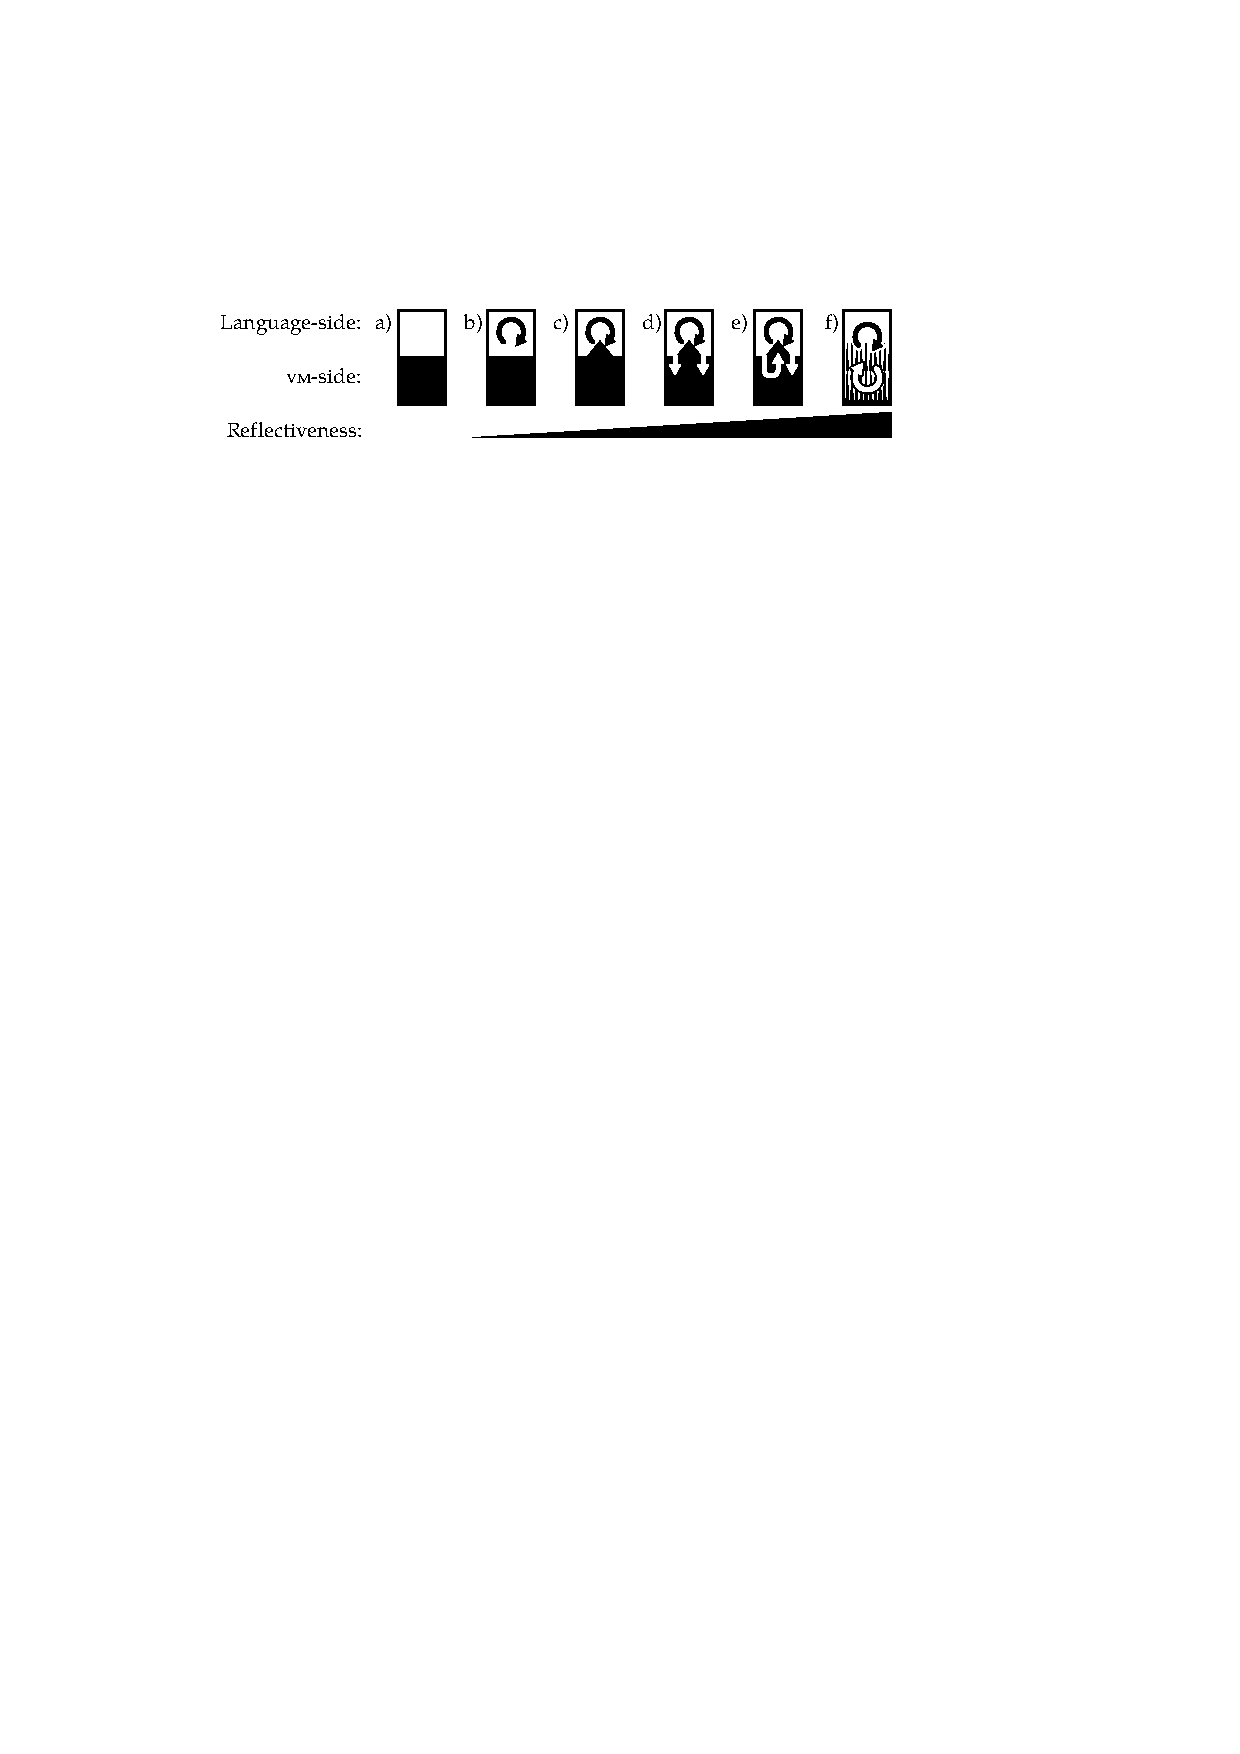
\includegraphics[scale=1.1]{vm-reflection-evolution}
	\figlabel{vm-reflection-evolution}
	\caption[High-level Language Reflection Evolution]{Evolution of reflection in high-level language runtimes.}
\end{figure}

\begin{enumerate}[a)]
\item \textbf{Language-side without reflection:}
	A language in this category requires a \VM to run but has no reflective properties.
	This includes early-stage languages such as the original Pascal-P system \cite{Nels79a}.
	This is rather an exception, since typically languages without reflection also lack the underlying \VM and are compiled to native code.
	Even with portability in mind it is possible to use for instance C as intermediate language which compiles under most platforms.
	
\item \textbf{Language-side with limited reflection:}
	The next step in the evolution of reflection is a language runtime with a \VM that support only certain static reflection.
	This might include structural reflection whose required information can be prepared upfront during the compilation phase.
	Such a system has no support for unanticipated reflection as there is no support from the \VM to dynamically reify concepts.
	A \VM with a \JIT in this category can perform strong optimizations and take full advantage of the runtime information.
	
\item \textbf{Language-side extended reflection:}
	The third category of high-level language runtimes has extended reflection with strong support from the underlying \VM.
	We put \PH, \ST implementations or \Self in this category of languages.
	The \VM supports complex reification of otherwise non-accessible concepts.
	Additionally we see 
	These language runtime support extended behavioral reflection for instance accessing and modifying the execution context.
	The supported reflective capabilities can not be anticipated, and thus require strong support from the underlying \VM.
	At this stage the \VM-level optimizations are a balance between restricting the supported language or sacrificing speed.
	
\item \textbf{Language-side introspection of the \VM:}
	The \VM support for reflection is highly extended compared to the previous category.
	Instead of a hidden property, certain \VM-level concepts are made explicitly accessible to the running language.
	Up to some extent this is similar to language-side structural reflection as the \VM only supports only a restricted interface which is defined at compile-time.
	In this category the language can only read (introspect) \VM properties.
	This might include reading out \JIT related properties such as performance counters or type annotations.
	Typically these operations are support by \VMs running in debug mode, which enables remote introspection.
	However, this does not imply that the language-runtime is capable of doing so reflectively.

\item \textbf{Limited language-side intercession of the \VM:}
	The previous category allows the language-side to safely read \VM-level properties.
	If we follow the same path as the language-side evolution of reflection the next step is to allow for modification at \VM-level.
	Such a language-runtime has a dynamic interface to change certain properties of the \VM.
	However, the \VM is still not fully reflective in the sense that not all \VM concepts are reified.
	This essentially limits the language-side to simple interactions and changes to the \VM itself.
	At this point the \VM can no longer guarantee safety by isolating the language-side from all the low-level details.
	Again no systems are known to fit in this category.
	\sm{Still to vague for my taste, and I still can imagine things I would put into this category}
	
\item \textbf{Self-aware \VM:}
	We classify in the last category dynamic language-runtimes that have no longer a clear separation of \VM and language-side.
	The same reflective properties equally apply to language-side and the \VM.
	The way to achieve this is by flattening out the intermediate \VM and let the language-side directly control everything.
	Currently there are several research \VMs which can be classified as self-aware \VMs: The \P \VM \cite{Verw12a} is partially self-aware but in control of the underlying execution and the \Klein \VM is fully reflective \cite{Unga05a}. 
	Unsurprisingly we find that these \VMs are built metacircularly, they are written in the same language they support.
\end{enumerate}

From this overview of the evolution of reflection in high-level languages and their \VMs we see that there certain language runtimes that provide a form of \VM-level reflection.
Which is a clear indicator that the clear separation between language-side and \VM-side is mostly incidental.
However, we see that there is only little research about self-aware \VMs or reflective \VMs.
According to our overview, only a few research language runtimes would classify as self-aware.
Combined with the previous two categories d and e, we see that metacircular \VMs encourage extended reflection.
In the following section we are now going to describe in more detail how metacircular \VMs are built and what their contribution to the high-level low-level interaction is.



% ===========================================================================
\section{Open \VMs}
\seclabel{background-open-vms}
% ===========================================================================

High-level language \VMs are inherent complex pieces of software.
They have to combine two rather extreme goals: abstraction and performance.
We have seen that the required abstraction for the running high-level language has a strong influence on the \VM design.
At the same time the hard performance requirement requires precise interaction with the underlying hardware.
This goes even so far that specialized hardware is conceived to match the performance requirements \cite{Unga84a,Stef84a,Clic05a}.
\todo{ref to java processor}

The early \VMs focused on interpreting an abstract instruction set (bytecodes).
The benefits are twofold.
On the one hand the bytecodes guarantee certain platform independence by abstracting away from the \CPU specific instruction set.
On the other hand bytecodes allow to encode complex operations into little space both serving the hard memory constraints of the hardware and simplifying the design of a compiler.
Obviously this abstraction gain comes at a cost and ever since the first \VMs were built research and industry strive to reduce the interpretation overhead.
An efficient way to improve performance is to use a just in time compiler (\JIT) that dynamically generates native code from the bytecode \cite{Deut84a}.
In this case the bytecode becomes an intermediate representation (\IR) for a bigger compiler infrastructure.
However, \JIT compilers are notoriously complex as they crosscut many \VM components.
At the same time they crosscut all abstraction layers; they have to access high-level information from the running bytecodes and manage native code at the same time.
Similar complexity applies to the automatic memory management present in most high-level language \VMs.
Garbage Collectors (\GC) evolved from simple helpers to complex software artifacts that for instance support concurrent garbage collection \cite{Clic05a}.

The increased complexity of the \VMs lead to more novel approaches on how to build \VMs.
\VMs are still build for a big part in C or C++ for performance reasons.
However, there are more high-level approaches that try to simplify creating \VMs by using building blocks \cite{Geof10a}.
\sm{Really? What is 26, I really need to jump through the PDF here? Not nice to your reader, not nice at all. If you got a point to make, make it explicit, not indirect. It is your text, you want to convey a message, do it precise and clearly, don't make me guess. If the point is not important, don't raise it.}
In the following sections we are shedding light on metacircular \VMs which are programmed in the same language they in the end support.

% ---------------------------------------------------------------------------
\subsection{Metacircular \VMs}
\seclabel{background-metacircular-vms}
% ---------------------------------------------------------------------------
The ever growing complexity of \VMs and the abstraction mismatch between the \VM definition language and the final interpreted language lead to a new movement that tried to reduce complexity.
Among the \VMs using higher-level languages or frameworks to reduce the development effort the metacircular building process stands out.
Unlike the classical \VM which is built in C and compiled to the a binary, a metacircular \VM is written in the same language that it provides in the end.
The following figure highlights the most evident differences between a classical and a metacircular approach.
%
\begin{figure}[h]
	\centering
	\vspace{1mm}
	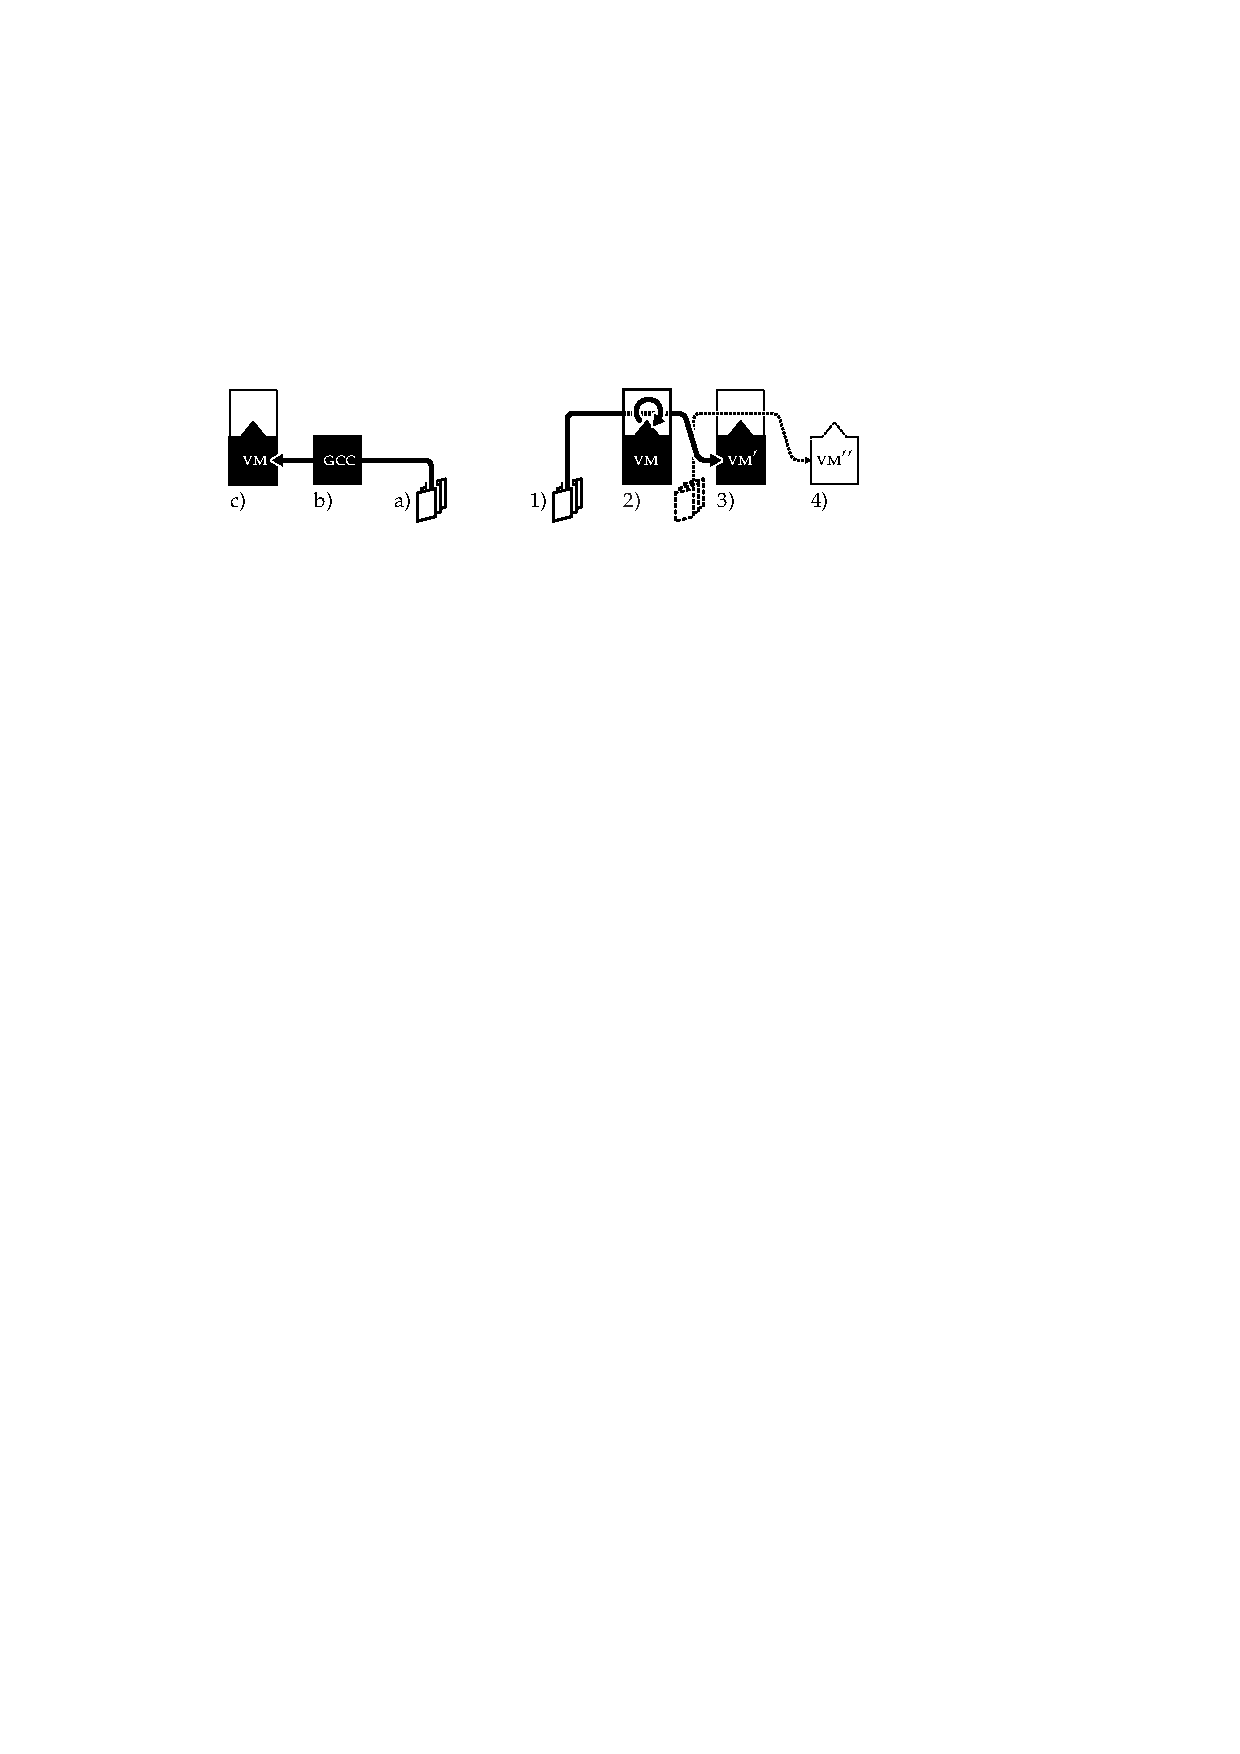
\includegraphics[scale=1.1]{vm-metacircular-building-process}
	\vspace{-5mm}
%	\figlabel{vm-metacircular-building-process}
\end{figure}
%
\begin{description}
\item[Classical \VM Compilation] \hfill
%	\sm{Why is the compilation process the thing you focus on? Isn't that incidental? }
	\begin{enumerate}[a), nolistsep]
		\item \VM sources typically written in C or C++
		\item Compilation of the \VM sources using a C or C++ compiler
		\item Final Binary
	\end{enumerate}

\item[Metacircular \VM Compilation] \hfill
	\begin{enumerate}[nolistsep]
		\item \VM sources written in a high-level language, the same as the final \VM supports
		\item Compilation of the \VM sources happens by evaluating the \VM sources, allowing for compile-time reflection
		\item New \VM' binary built using an existing version of the \VM
		\item The new \VM Binary can be used to compile again a new \VM''
	\end{enumerate}
\end{description}

\noindent Using the same language for developing the \VM has several advantages.
Usually the \VM is in great contrast to language-side libraries on the same platform.
This is due to the low-level nature of the \VM.
Using a high-level language certain implementation details can be hidden.
Furthermore the metacircular approach provides the \VM developer with the same tools as a language-side programmer.
Typically this leads to faster development.


Inside the metacircular \VM community we see different approaches with varying levels of abstractions and reuse.
When compared, we find differences in how metacircular \VMs build \VM components (\GC, \JIT) and how the bootstrap or compilation of the new \VM works.
We see metacircular \VMs that use the high-level language as an advanced macro systems.
In a sense an extended version of C++'s templates.
Other approaches use the full reflective power of the high-level runtime to simplify code.
And even more advanced system automatically provide the \VM developer with \GC or a \JIT compiler.
We will now elaborate in more detail how metacircular \VMs are constructed.


\paragraph{Language Property Synthesis}
In the classical C-based \VM approach all \VM components have to be explicitly build.
Each \VM is a one of a kind with custom interpreter and a specialized memory manager.
Using high-level \VM frameworks it is possible to provide the \VM developer with prefabricated components.
For instance it is possible to simply parametrize a premade \GC to reduce development effort.
Looking at the evolution of metacircular \VMs we see both approaches.
For instance pseudo metacircular solutions like the \Squeak \VM \cite{Inga97a} work more like a high-level C macro system.
The high-level language is used to generate C code which is then further compiled to the final \VM binary.
\VM components are declared in a very explicit style, again not much different from C++.
Memory for \VM-level structures has to be managed in the same way as its C++ counterpart by explicitly allocating and freeing objects.
On the other side we have \VM frameworks like \PyPy for the \Python language that provide automatic \GC and \JIT support.
Here the developer writes a new \VM in almost the same way as a normal \Python program.
In the ideal case only certain hints are necessary to create a \JIT.

\todo{Truffle as extreme to that track: Interpreter implementation on \AST basis, not explicit bytecode interpreter (which would be typical in C)}

\paragraph{Bootstrap Process}
\sm{And by the way, I forgot where you are going with all this. Why do I care about the bootstrap process?}
A crucial step during the development with the metacircular \VMs is the bootstrap of the new \VM.
We distinguish mainly between two approaches, indirect bootstrap and direct bootstrap.
%
\begin{figure}[h]
	\centering
	\vspace{2mm}
	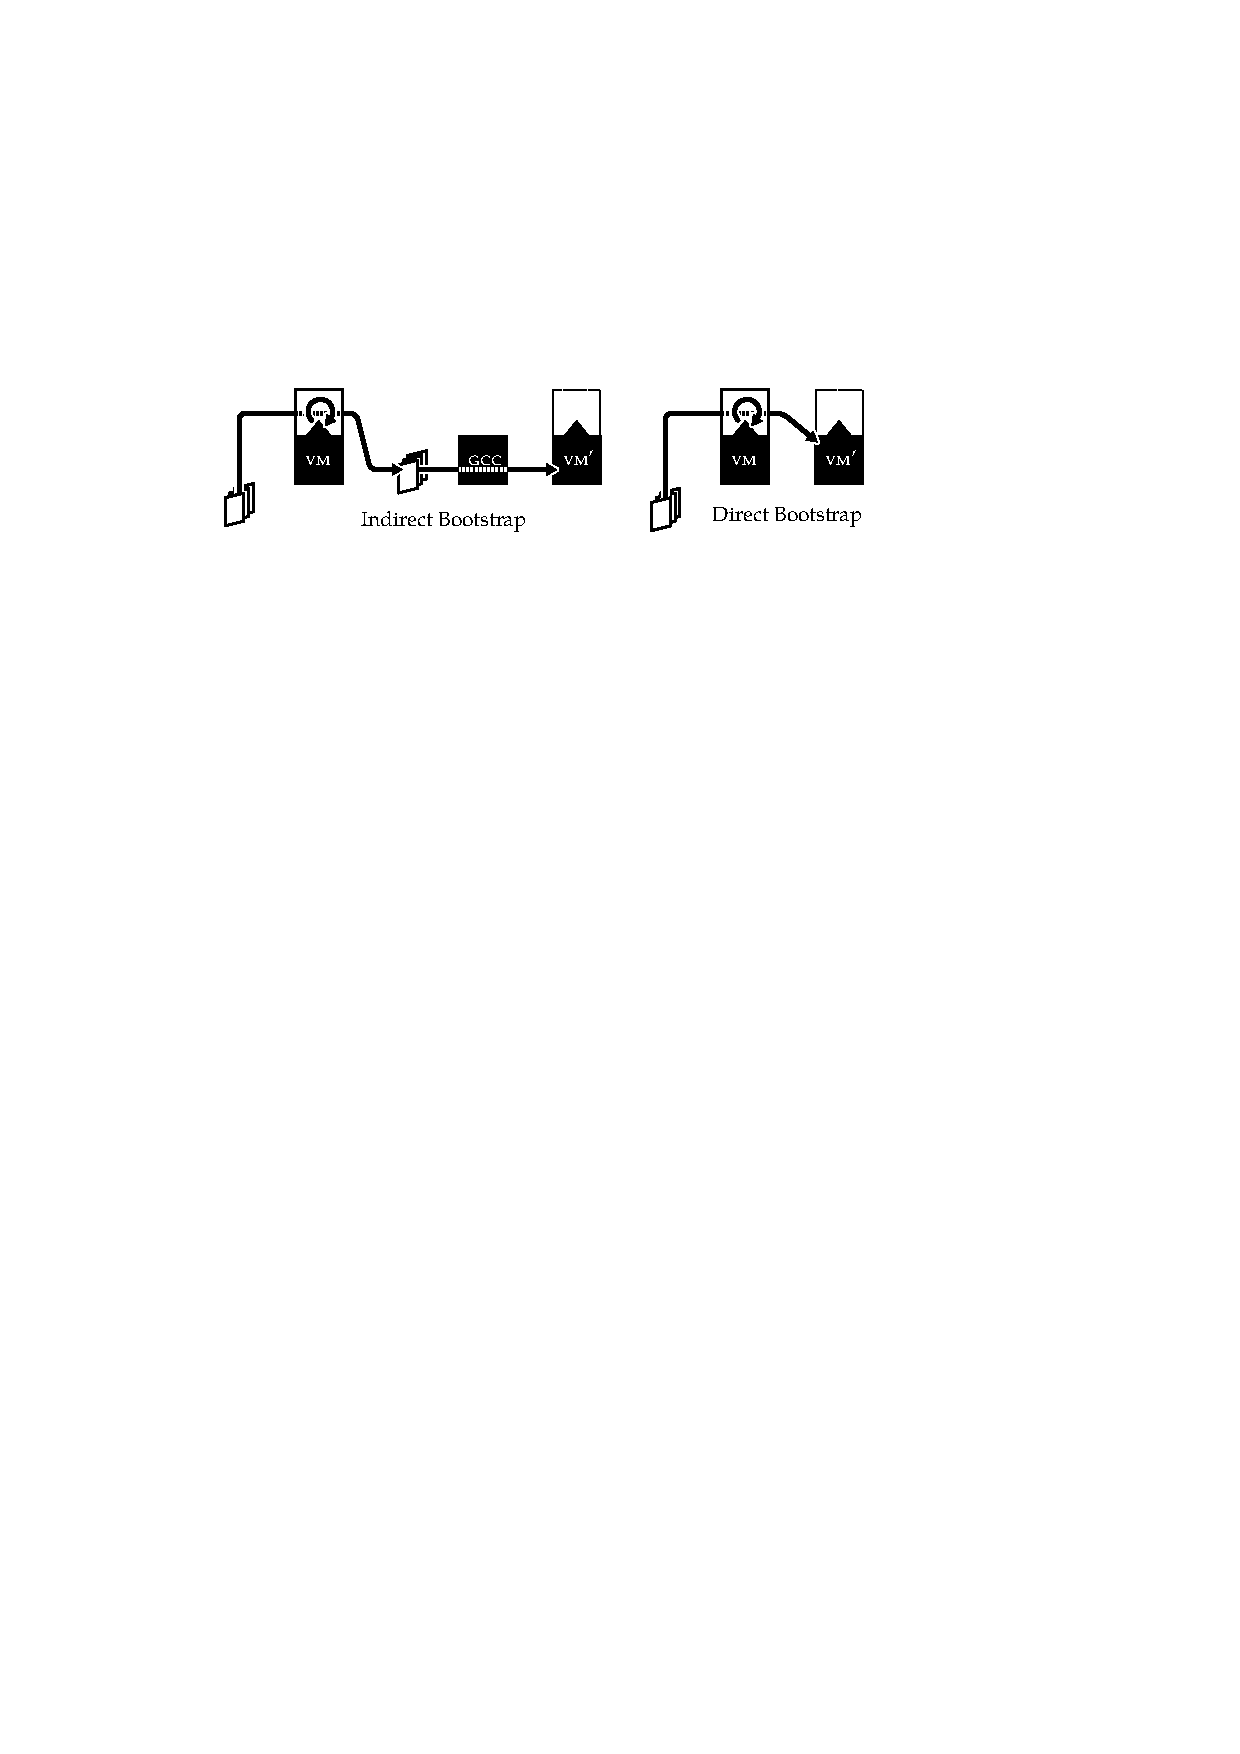
\includegraphics[scale=1.1]{vm-metacircular-bootstrap}
	\caption{Metacircular \VM Bootstrap Types}
	\vspace{-5mm}
	\figlabel{background-metacircular-bootstrap}
\end{figure}
%
\begin{description}
\item[Indirect Bootstrap:]
	Metacircular \VMs with an indirect bootstrap use an intermediate language to compile a new \VM binary.
	A typical example of this approach is \Squeak and \PyPy using C.
	Both of these system imply a complete C compilation stack.
	The advantage of this approach is the that C is heavily optimized thus reducing the development effort for the \VM framework.
	However, C already hides a lot of low-level details away.
	Typically the \VM framework has to work around these limitations when working directly with native code for instance in the \JIT.
	We have explicitly seen these limitations while working on the \P \VM.
	
\item[Direct Bootstrap:]
	Metacircular \VMs with a direct bootstrap are directly in charge of generating the native code for the final binary.
	We have seen in \P that many C-level optimizations have only limited impact on the final speed.
	A major speedup is achieved by using a native stack and directly generating native code instead of using a bytecode interpreter.
	Hence the \VM will probably require an assembler framework which in return can be used for the direct bootstrap.
	This means that only limited additional efforts are necessary for a direct bootstrap.
	As a result the direct bootstrap allows full control of how the final binary will look like.
	\sm{Neither using the stack directly, nor generating native code is specific to direct bootstrapping, it is entirely orthogonal. Your discussion and examples here are not consistent with the goal I perceive for this section }
\end{description}

% ---------------------------------------------------------------------------
\subsection{Compile-time Reified \VMs}
% ---------------------------------------------------------------------------
\sm{My questions at a beginning of a section are: why do I read it? What am I going to learn? And how does it fit with/supports the thesis goal?}
After presented the technical background of metacircular \VMs we are presenting several concrete implementations in more detail.
In this first part present \VMs that focus on compile-time reflection.
In \secref{background-reified-vms} we will then focus on a list of \VMs that reify their components and allow for a more close interaction with the language-side.


\subsubsection*{\Squeak \ST \VM}
\seclabel{background-squeak}
% ---------------------------------------------------------------------------
\sm{I still don't take squeak as metacircular in the strict sense. For me, that means  implemented in itself. Java with java, lisp with lisp, smalltalk with small talk, squeak is implemented in slang, that's C with smalltalk syntax, which is barely executable as smalltalk, PyPy is implemented with RPython, also restricted subset, and with its type system, I would say, a very different language. You can however make the point that RPython is a strict subset of Python, and thus, without changes directly executable. That's not true for Slang...}
The pseudo metacircular \Squeak \VM\cite{Inga97a} is of importance in the context of this work.
Its core building system is still in active use for the \urlfootnote{\Cog \VM}{http://www.mirandabanda.org/cogblog/} which extends \Squeak with a \JIT.
The \Cog \VM is used as default by the \urlfootnote{\PH}{http://pharo.org/} programming language.
\Squeak is built around a \ST dialect called \Slang that is exported to C to be compiled to the final \VM binary.
Additionally the \Slang sources can be interpreted to provide an interactive simulator of the \VM, including full graphical support.

\Slang is limited to the functionality that can be expressed with standard C code.
\Slang in this case is mostly a high-level C preprocessor.
Even though \Slang basically has the same syntax as \ST it is semantically constrained to expressions that can be resolved statically at compilation or code generation time and are compatible with C.
Hence \Slang's semantics are closer to C than to \ST.
Unlike later metacircular frameworks \Squeak uses little or no compile-time reflection to simplify the \VM designs.
However, class composition help structuring the sources.
Next to the \Slang source which account for the biggest part of the interpreter code some \OS-related code and plugins are written in C.
To facilitate the interaction with the pure C part \Slang supports inline C expressions and type annotations.
\sm{Why is all of this important here? Does not seem to contribute to your discussion }

A great achievement of the \Squeak \VM is a simulator environment that enables programmers to interact dynamically with the running \VM sources.
The simulator is capable or running a complete \Squeak \ST image including graphical user interface.
This means that programmers can change the sources of the running \VM and see the immediate effects in the simulator.
The simulator itself works by setting up a byte array which servers as native memory.
Then the \VM sources written in \Slang are interpreted by the \VM of the development environment.

We see that \Squeak is a pseudo metacircular \VM that uses an indirect bootstrap process.
The newly created \VM does not absorb any features from the host environment.
Yet according to long-time \VM programmers the \Squeak infrastructure is more productive than a comparable C++ or pure C project.

% ---------------------------------------------------------------------------
\subsubsection*{\Jikes: High-level low-level Programming in with \MMTK}
\seclabel{background-jikes}
% ---------------------------------------------------------------------------
\Jikes (former \textsc{Jalapeño})is an early metacircular research \VM for \Java \cite{Alpe00a}.
The \Jikes \VM features several different garbage collectors and does not execute bytecodes but directly compiles to native code.
With metacircularity in mind \Jikes does not resort to a low-level programming language such as C for these typically low-level \VM components.
Instead they are written in \Java as well using a high-level low-level programming framework.

The \Jikes \VM had performance as a major goal, hence direct unobstructed interaction with the low-level world is necessary using a specialized framework.
High-level low-level programming \cite{Fram09a} is mentioned the first time in the context of the \Jikes \VM project.
The goal of high-level low-level programming is to provide high-level abstractions to simplify low-level programming.
Essentially this is the same motivation that drives the metacircular \VM community.

Frampton et al. present a low-level framework packaged as \ttt{org.vmmagic}, which is used as system interface for Jikes, an experimental \Java \VM.
Additionally their framework is successfully used in a separate project, the memory management toolkit (\MMTK) \cite{Blac04a} which is used independently in several other projects.
The \ttt{org.vmmagic} package introduces highly controlled low-level interaction in a statically type context.
In their framework, methods have to be annotated to enable the use of low-level functionality.

% ---------------------------------------------------------------------------
\subsubsection*{\Maxine \Java \VM}
\seclabel{background-maxine}
% ---------------------------------------------------------------------------
\Maxine is a metacircular \Java \VM \cite{Wimm13a} focused on an efficient developer experience.
Typically \VM frameworks focus on abstraction at the code-level which should yield simpler code and thus help reducing development efforts.
However, in most situations the programmer is still forced to use existing unspecific tools for instance to debug the \VM.
In contrast to that, the \Maxine \VM provides \ugh{first-hand tools} to interact with the \VM in development.
\Maxine uses abstract and high-level representations of \VM-level concepts and consistently exposes them throughout the development process.
Inspectors at multiple abstraction levels are readily available while debugging, giving insights to the complete \VM state.
\Maxine provides and excellent navigation for generated native code by providing links back to language-side objects as well as other native code and symbols.

Even though the \Maxine projects follows an approach where reflection is only used at compile-time, the development tools themselves provide a live interaction with the running \VM artifact.
However, the \VM itself is not reflective as it is not directly built to reason about itself.
This means that when debugging the \VM it behaves almost like a life \ST image where a complete interaction with the underlying system is possible.
We identify this as crucial, as most of the time is spent debugging, notably on inadequate tools like \ttt{gdb} due to lack of alternatives.
\sm{Connect this to your problem statement (back reference) and, make sure your problem statement does not mix up reflection and observability/interactivity }
Hence having a specific debuggers and inspectors greatly improve the interaction with the \VM artifact.

\subsubsection*{\PyPy Toolchain}
\seclabel{background-pypy}
% ---------------------------------------------------------------------------
\urlfootnote{\PyPy}{http://pypy.org/} is a \Python-based high-level \VM framework \cite{Rigo06a}.
\PyPy's major focus lies on an efficient metacircular \Python interpreter.
However, it has been successfully used to build \VMs for other languages including \ST \cite{Bolz08a}.
Interpreters are written in a type-inferable subset of \Python called \RPython.
The underlying \PyPy infrastructure implicitly provides memory management and \JIT compilation.

\PyPy follows a different approach from the previously presented \VM generation frameworks.
For instance, in Squeak and \Jikes the final \VM implementation is not much different from C or C++.
\sm{C/c++ has nothing to do with this

It is about direct implementation vs. composition by a tool chain or something similar. At least that's my understanding here}
The programmer specifies all the components of the \VM explicitly, either by implementing them directly or using a provided library.
Compared to the more static C ans C++ these \VM generation frameworks make the compilation phase more tangible.
\ST in \Squeak or \Java in \Jikes or \Maxine fulfill the purpose of the template system in C++ or the restricted macro system in C.
For the explicit implementation part \PyPy is no different.
However, certain features for the final \VM are directly absorbed from the underlying \PyPy infrastructure.
For instance, the \JIT support or the \GC are not explicitly implemented but provided by the \PyPy framework itself.
This is a big difference to the other \VM frameworks as it allows programmers to write the \VM in a more high-level fashion.
For instance in \Squeak memory allocation, even for \VM-level objects, has to be handled in the same way as in C.
Whereas in \PyPy the garbage collection is left to the underlying infrastructure.
\sm{This paragraph needs to be revised, your line of argumentation is confusing/conflating many different aspects, and that does leave a bitter taste to me as a reader}

At compile-time the interpretation stack for a newly implemented \VM on top of \PyPy looks as follows.
\sm{Why do I care for those details?}
%
\begin{enumerate}[noitemsep,nolistsep]
\item The final language runtime
\item The \VM written in \RPython
\item The \PyPy infrastructure (virtual compile-time \RPython interpreter)
\sm{These terms don't mean anything to me? Which part is which? What's the implemented language? Concrete example?}
\end{enumerate}
%
Unless in debug mode, the bottom-most layer is compiled away by exporting the \RPython sources to C.
However, before the C export step, all the compile-time reflection statements are evaluated and flattened away.
This approach allows \RPython \VMs to behave almost like standard \Python programs while still providing excellent performance in the final \VM binary.

Much like the automatic memory management, \PyPy provides a tracing \JIT generator \cite{Bolz09a}.
By default the \VM programmer does not write an explicit \JIT in \PyPy.
Instead the \VM code is annotated to guide the underlying tracing \JIT generator.
This means a \VM compilation time a specific tracing \JIT is created for the given meta information.
As a result, the \JIT can track high-level loops in the final interpreted language.
\sm{What's the similarity between GC and tracing JIT? One traces object graphs the other traces operations, two totally different things

Aaaaah, it is provided as a service, implicitly, ...
Ok, make that explicit, say something like that}


% ---------------------------------------------------------------------------
\subsection{Runtime Reified or Self-aware \VMs}
\seclabel{background-reified-vms}
% ---------------------------------------------------------------------------

The \VMs presented so far have little or no self-awareness.
\VM generation frameworks allow a high amount of reflection at \VM compile time.
This meta information is typically compiled away.
This is somewhat similar to what happens with templates in a C++-based \VM.
The \VM frameworks themselves behave like a static language on their own.
As a result, the final \VM artifact has no access to the underlying definition anymore.

As an example we might have several \VM components represented as high-level objects at compile or \VM generation time.
These objects have a class and methods attached, information that is reflectively accessible.
However, once the \VM is compiled down to native code, most of this information is lost.
What is left is native code with low-level instructions that allow little or no reasoning about the original high-level structure.
\sm{This is way to general and unspecific, and  I am not sure why that's discussed here}

We have shown in \secref{background-vm-reflection} how a potential evolution of reflection in a high-level language looks.
We concluded that the evolution of language-side reflection implies a similar evolution at \VM-level.
More behavioral reflection at language-side requires more concepts to be reified in the \VM itself.
This requirement is conflicting with the previously described loss of reification at \VM-level.

We are now going to present \VMs that behave significantly different.
Unlike the previous ones, they no longer make a clear distinction between the static \VM and the dynamic language-side.


% ------------------------------------------------------------------------------
\subsubsection*{\DwarfPython}

\DwarfPython \cite{Kell11a} is a \Python implementation that aims at a barrier-free low-level interaction.
It emerged from an earlier \textsc{Parathon} which used \Dwarf debugging information from external libraries to facilitate foreign function interfaces.
\DwarfPython takes this idea further.
Additionally to describe low-level code, \DwarfPython uses the \Dwarf metamodel to describe \Python code and data.
This is depicted in \figref{background-dwarf-python}.
%
\begin{figure}[h]
	\centering
	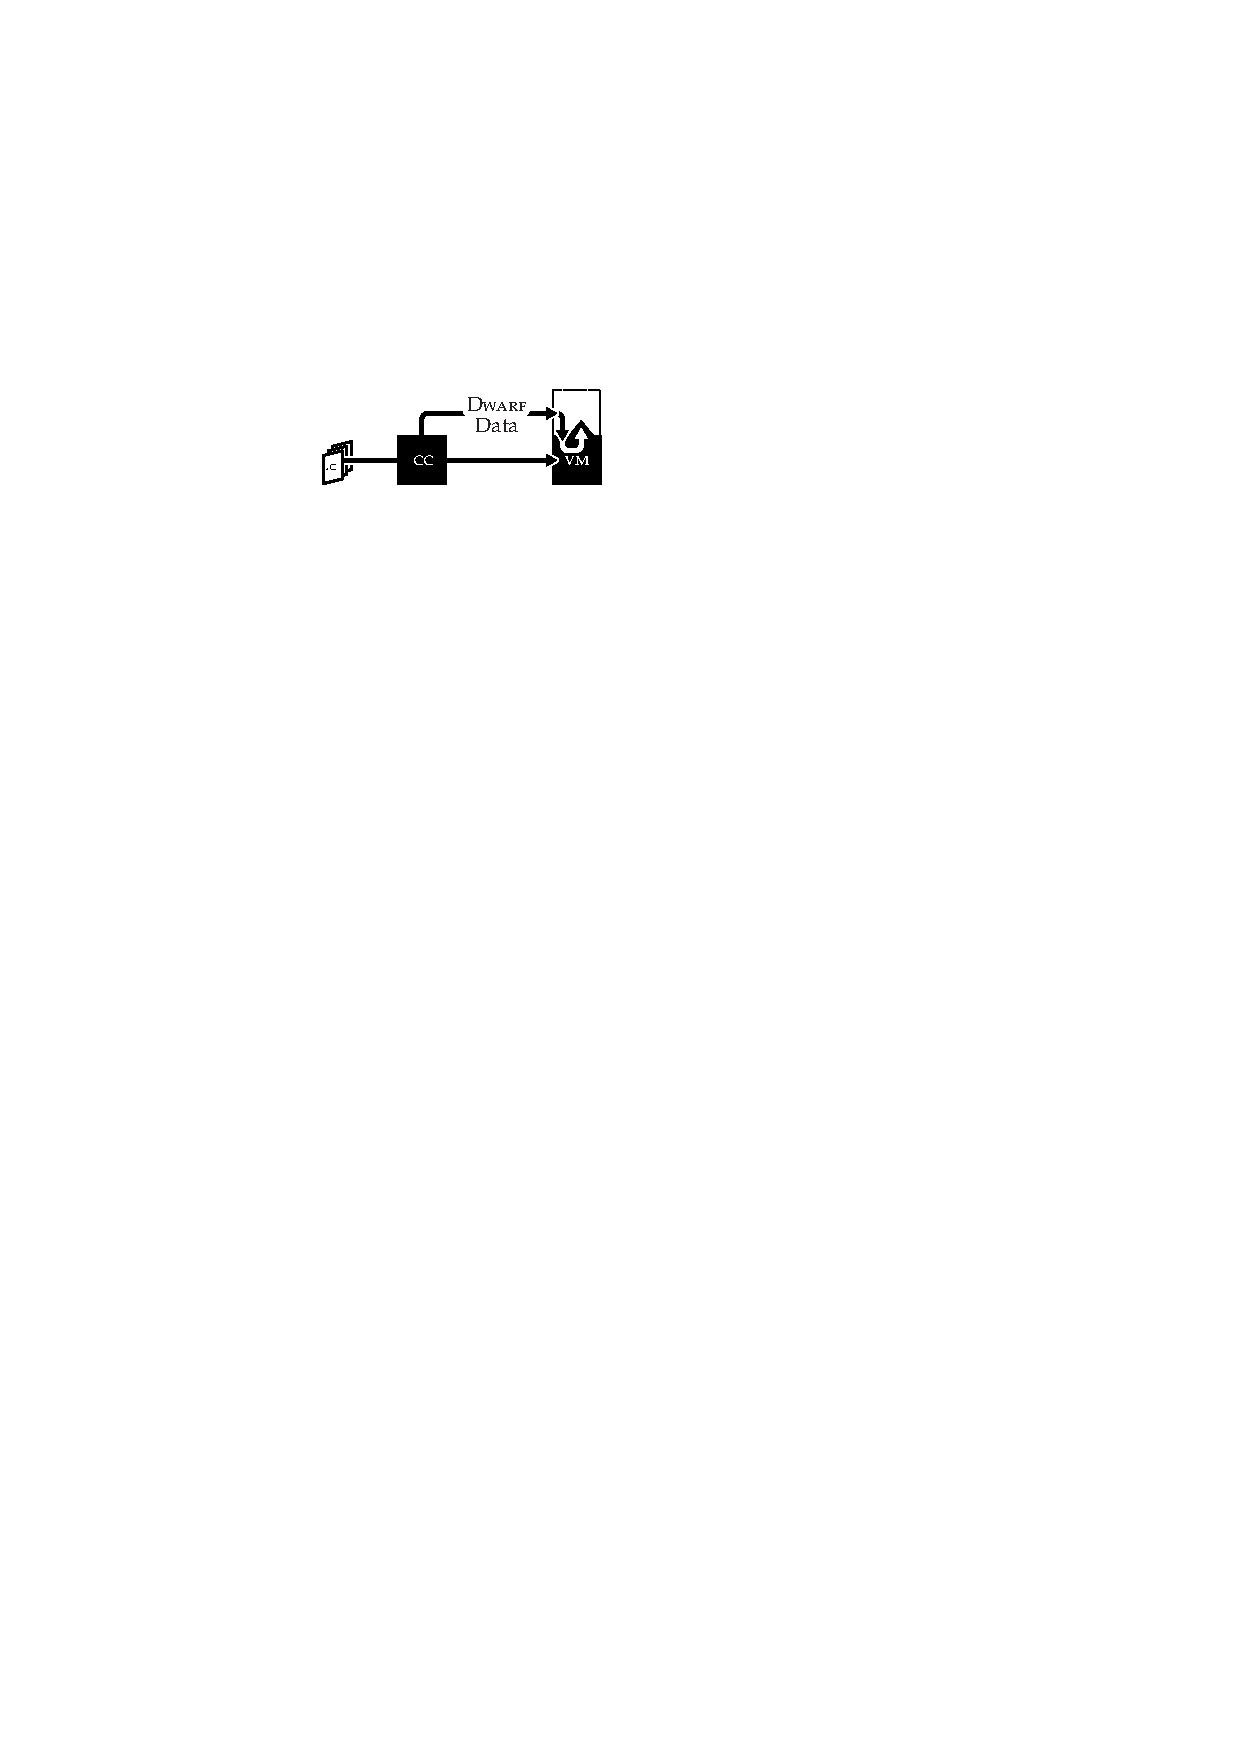
\includegraphics[scale=1.1]{vm-dwarf-python}
	\caption[\DwarfPython Low-level Reification]{\DwarfPython reifies the low-level \VM by using the \Dwarf Debugging information at language-side.}
	\figlabel{background-dwarf-python}
\end{figure}
%
This approach has the advantage that the very same debugging mechanism applies for low-level code, for instance written in C, and for high-level \Python code.
Thus \DwarfPython essentially unifies the previously decoupled \VM with the language-side.

% ------------------------------------------------------------------------------
\subsubsection*{\Pinocchio \VM}
\seclabel{background-pinocchio}

\P \cite{Verw11a} is a research \ST environment that directly uses native code instead of bytecodes.
The only execution base is native code which is directly generated by the language-side compiler.

\P is built from a kernel derived originally from a \PH image.
For the bootstrap classes, objects and methods are exported into binary, native images and linked together with a standard C linker to a final executable.
For simplicity we also rely on a very small part of C code to provide essential primitive, for instance used for file handling.
Additionally we specified part of the bootstrap for the \ST object model in plain C code.
However, besides that, all the other code is written and developed directly in \ST.
%
\begin{figure}[h]
	\centering
	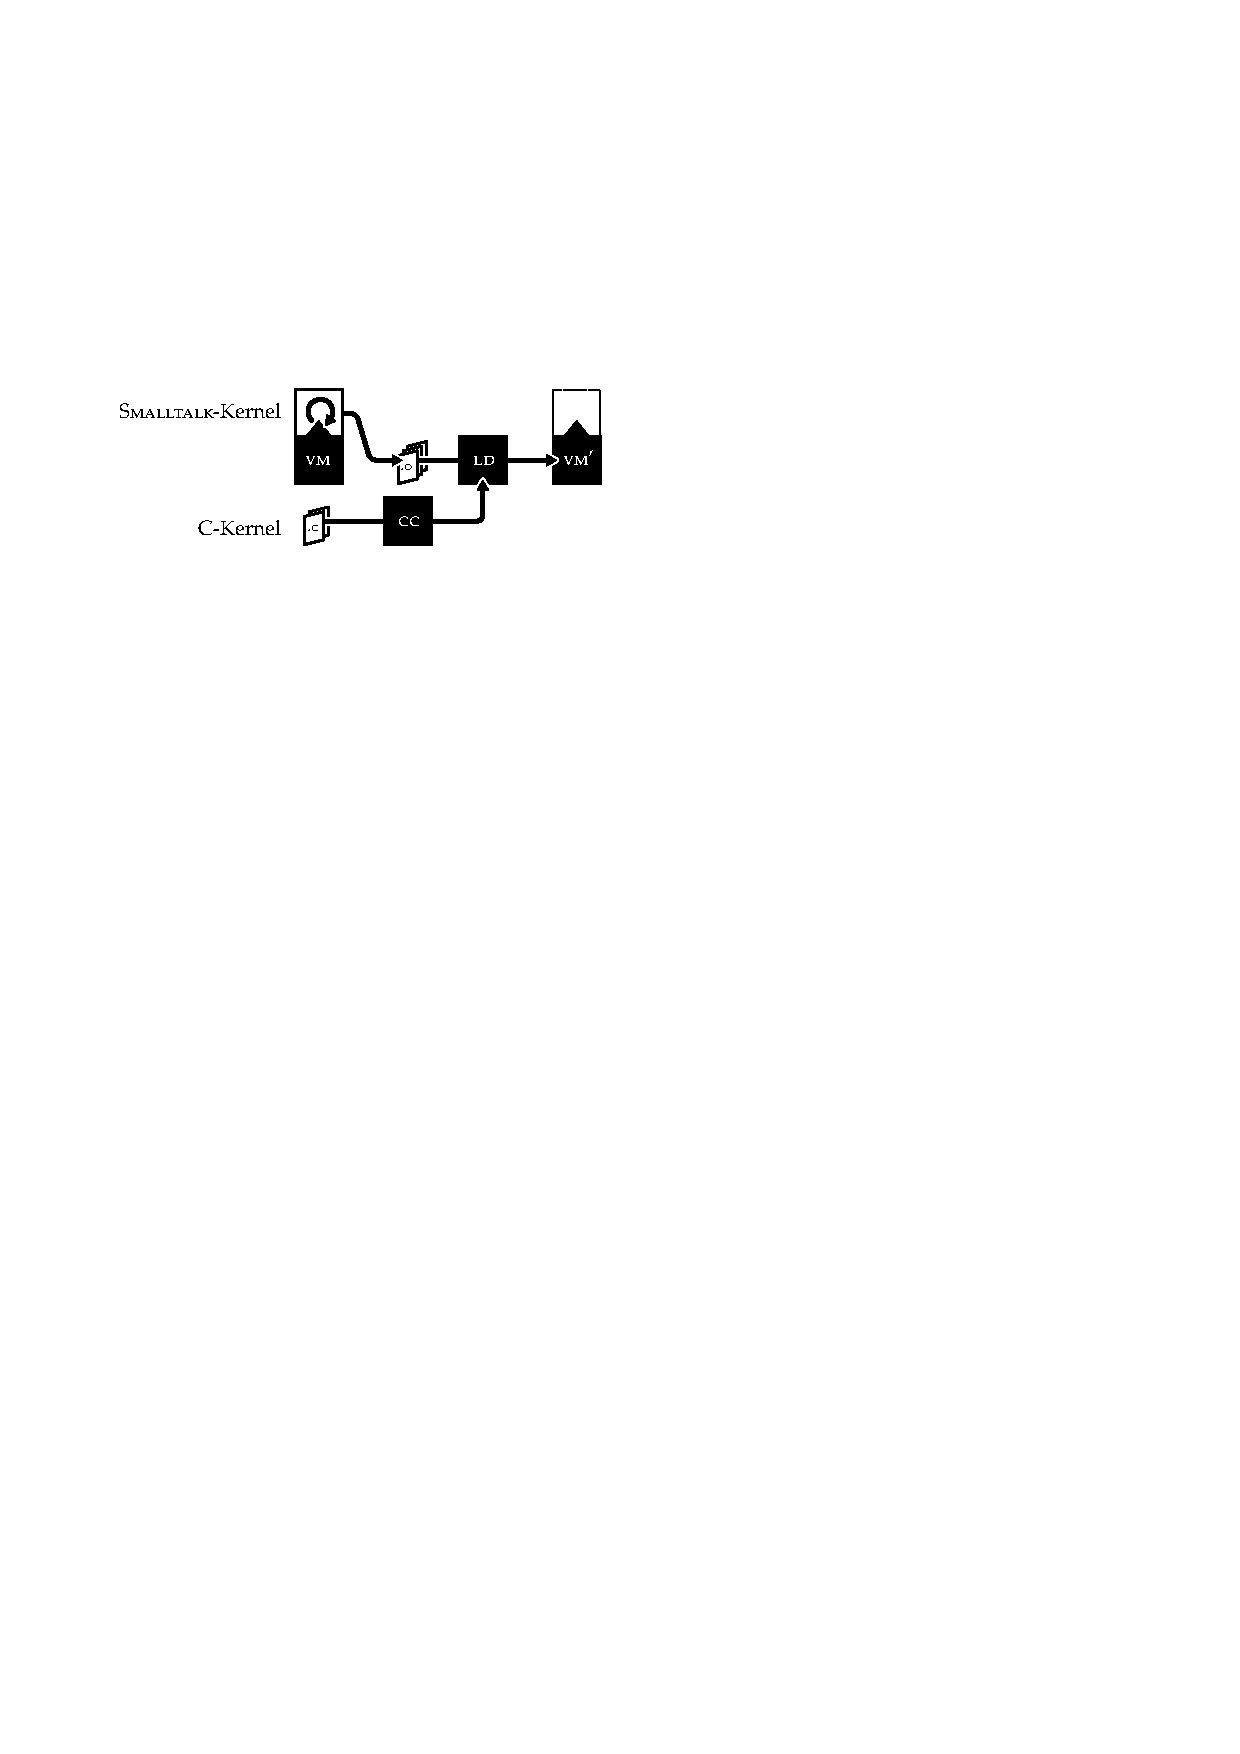
\includegraphics[scale=1.1]{vm-pinocchio-bootstrap}
	\caption{\P's Bootstrap}
	\figlabel{background-pinocchio-bootstrap}
\end{figure}

An important aspect of \P is that the method lookup is expressed in terms of normal \ST code.
Typically this code statically resides in the \VM, thus at a different meta-level.
Hence this implies for most systems that the lookup can not be modified without altering the \VM itself.
However, expressing the lookup in terms for normal language-side code introduces a recursive dependencies during the bootstrap.
In order to run the lookup code expressed in \ST code, we have to perform message sends.
These, in return, require an already working lookup mechanism.
Hence, without a taking special care, a language-side lookup method will lead to infinite recursion during startup.
We resolved this problem in \P by directly interacting with the low-level execution format which among other things relies on inline caches to improve performance.
The important property of inline caches is that they bypass the slow language-side lookup by directly jumping to the last activated method at a send-site.
This is exactly the behavior we need to prevent recursion during the startup.
Hence, when generating the native code for the bootstrap, we prefill all the inline caches of the methods required to perform a full method lookup.
As a result, when running requiring the first real method lookup, the lookup code itself is running perfectly on the prefilled inline caches.
\sm{Ok, cool, how is that relevant in this context?}

From an architectural point of view, \P is performing almost a direct bootstrap.
Besides the small C kernel, the language-side code is directly compiled to native code.
As a result, \P only requires a single compiler for native code, during bootstrap and at runtime.
Hence, a separate \JIT implementation is not required.

The most obvious shortcoming of \P is the lack of its own garbage collector.
Instead of investing time into a separate well-defined \GC \P relies on the conservative \urlfootnote{Boehm \GC}{http://www.hpl.hp.com/personal/Hans_Boehm/gc/} built for C programs.
The Boehm \GC is sufficiently fast to run \P as a prototype, however, due to its generic nature it is not as efficient as a specific \GC.
However, \P lacks the necessary reification at level of the object layout to properly implement a \GC.
\sm{Why does that matter? And why is 'efficiency' relevant  here?}
All the notion about the object layout in memory are hard-coded in the compiler in several places.
Work was undertaken to put first-class object layouts in place and delegate memory allocation and field access to these meta objects.
Yet, at the current state \P has not incorporated this in the compiler core.
\sm{The whole section over and over again, you are first talking about something that's on its own only barely relevant, and then afterwards you make it relevant to me as a reader. Your writing could improve a lot by following classic paragraph structure: title sentence, main argument,mans then details and/or examples + supporting arguments.

To proof your thesis is your only goal, I would prefer if everything is explicit or at least implicitly written to make }

\P is self-aware in the sense that it controls  native code generation and lookup at a single abstraction level.
There is no distinction between \VM-level code and language-side code.
\sm{What does generation and modify ability of inline cache content have to do with self-awareness? his is still unclear to me, generation especially, reflecting on inline caches, I do understand. 

I have the feeling the conceptual model you outline in the beginning needs more elaboration and details.

And the criteria then could benefit this discussion to make it more precise (a few back references)}

% ------------------------------------------------------------------------------
\subsubsection*{\MIST a C-less \ST Implementation}
\urlfootnote{\MIST}{http://mist-project.org/} is another prototype \ST \VM that follows similar goals as the \P \VM.
As well, it no longer uses a bytecode interpreter but only relies on native code.
However, it goes one step further than \P by not relying on any C-based infrastructure.
\MIST implements its own linker to build the final executable.
Hence unlike \P it does not require kernel primitives written in C.
\MIST brings its own implementation to directly perform system calls from within the language.
\sm{Why is it relevant? It is barely a paragraph, feels like it doesn't fit in or is underrepresented here. Also, instead of being indirect about the goals, it would help to restate them}

% ------------------------------------------------------------------------------
\subsubsection*{\Klein \VM}
\seclabel{background-klein}

\urlfootnote{\Klein}{http://kleinvm.sourceforge.net/} is a metacircular \VM for the \Self programming language that has no separation into \VM and language \cite{Unga05a}.
\Klein performs a direct bootstrap (see \figref{background-metacircular-bootstrap}) much like the aforementioned \P or \MIST \VM.
Hence \Klein does not use an intermediate low-level language to bootstrap the system.
\sm{I still don't get the point about the low-level IR/byte code being one of the hints you pick on.

It is an exchange format, a serialization, what ever, I think you want to make the point that it is not being executed? Well, I am not to sure about that for Klein...}

It is important to point out that the \VM-level structures and objects are not compiled away as it is usually the case.
Instead the \VM structures are represented as real \Self objects.
Hence the \Klein \VM supports true \VM-level reflection since there is only a single code base.
\sm{I don't like the 'compiled away'. In hotspot, everything is a C++ object! no? I think, you'll probably have clarified that point in text that comes earlier, so, I would avoid such 'sloppy' language here and use the precise criterion/terminology from earlier}

Additionally to the advances in reflection and metacircularity, \Klein focuses on fast compilation turnarounds to allow for a responsive development process.
Which is unlike for instance the \Squeak \VM where a full \VM bootstrap takes an order of minutes on modern hardware.
\Klein also supports advanced mirror-based debugging tools to inspect and modify a remote \VM.

Development on the \Klein \VM seized in 2009 and left the \Klein \VM in fairly usable state.
Like \P it currently lacks a dedicated \GC.
Yet, it proved that it is possible and build a language-runtime without a proper separation of the language-side and the \VM or base-level.
\sm{Proper is the wrong word here, proper has a positive connotation, also implying it is necessary}
From the literature presented about the \Klein project we see a strong focus on the improvements of the development tools.
The fact that the language-runtime allows \VM-level reflection to change the \VM dynamically is not directly mentioned in the literature.
While we see the practical limitations of changing the \VM at runtime we would like to open the doors to this new form of reflection.


% ===========================================================================
\section{High-level Low-Level Applications}
\seclabel{background-high-level-low-leve-application}
% ===========================================================================
% ---------------------------------------------------------------------------
\subsection{Foreign Function Interfaces (\FFI)}
\seclabel{background-ffi}
\seclabel{ffi-relatedWork}
% ---------------------------------------------------------------------------

Typical \ST system are isolated from the low-level world and provide only limited interoperability with C libraries.
However there are notable exceptions: \textsc{Étoilé} and \ST/X.

Chisnall presents the Pragmatic \ST Compiler \cite{Chis12a}, part of the \textsc{Étoilé} project, which focuses on close interaction with the C world.
The main goal of this work is to reuse existing libraries and thus reduce duplicated effort.
The author highlights the expressiveness of \ST to support this goal.
In this \ST implementation multiple languages can be mixed efficiently.
It is possible to mix Objective-C, \ST code.
All these operations can be performed dynamically at runtime.
Unlike our approach, \textsc{Étoilé} aims at a complete new style of runtime environment without a \VM.
Compared to that, \NB is a very lightweight solution.

Other dynamic high-level languages such as \Lua leverage \FFI performance by using a close interaction with the \JIT.
\urlfootnote{\LuaJIT}{https://github.com/jmckaskill/luaffi/} for instance is an efficient \Lua implementation that inlines \FFI calls directly into the \JIT compiled code.
Similar to \NB this allows one to minimize the constant overhead by generating custom-made native code.
The \LuaJIT runtime is mainly written in C which has clearly different semantics than \Lua itself.

On a more abstract level, high-level low-level programming \cite{Fram09a} encourage to use high-level languages for system programming.
Frampton et al. present a low-level framework  which is used as system interface for \Jikes, an experimental \Java \VM.
However their approach focuses on a static solution.
Methods have to be annotated to use low-level functionality.
Additionally the strong separation between low-level code and runtime does not allow for reflective extensions of the runtime.
Finally, they do not support the execution and not even generation of custom assembly code on the fly.

Kell and Irwin \cite{Kell11a} take a different look at interacting with external libraries.
They advocate a Python \VM that allows for dynamically shared objects with external libraries.
It uses the low-level \textsc{dwarf} debugging information present in the external libraries to gather enough metadata to automatically generate \FFIs.


% ---------------------------------------------------------------------------
\subsection{Just-in-time Compilation}
\seclabel{background-jit}
\seclabel{val-nabujito-related-work}
% -----------------------------------------------------------------------------
\todo{check for reference to \NBJ}
There is a vast amount of scientific literature when it comes to \JIT optimizers.
However, they focus on the optimization opportunities itself such as different compilation strategies or an efficient \GC interaction.
In the context of our work the compiler-based optimization are of second importance since we focus on the hybrid nature of a system that interacts with the low-level \VM world.

Jan Vran\'{y} et al. present a \ST with an explicit meta-object-protocol allowing for method lookup customization at language-side\cite{Vran12a}.
Their customized \ST/X \VM has an extended lookup mechanism where each class can specialize the lookup with a user definable \ttt{LookupObject}.
Hence for each message send the \VM first checks if the receiver's class provides a \ttt{LookupObject}.
By default this is not the case and the \VM falls back to the standard hierarchical \ST method lookup which is hard-coded in the \VM.
However, if the receiver class returns a proper \ttt{LookupObject} the \VM delegates the lookup to this user-defined object.
The \ttt{LookupObject} is invoked with context information about the message send including access to the low-level lookup cache.
While the other context information is important for new lookup schemes, the exposed cache provides an simplistic interface for the \JIT.
If the language-side lookup uses the provided cache it is still possible to implement efficient caching at \VM-level.
\todo{I don't think there is anything closer?}


A similar, albeit simpler approach, was provided in the research \ST \VM \P \cite{Verw12a}.
There the message lookup is fully implemented at language-side, but unlike the \ST/X solution only the context information required for a standard \ST lookup is provided.
More explicitly, \P does not provide access to an internal cache which could be used for speeding up more elaborate lookup customizations.

The two projects presented only implicitly deal with the \JIT interaction.
However, they provide evidence about high-level customizations for a part of the execution.
In both projects it is possible to dynamically customize a static core \VM concept.
While it is possible to modify the lookup mechanism in many \VM generation frameworks, this does not extend to the runtime

% ===========================================================================
%\newpage
\section{Problem 1: Dynamic High-level Low-level Programming}
% ===========================================================================
We have seen in the presented \VMs that a tight integration with the low-level code is indispensable.
Relying on an intermediate solution such as C with inlined assembler expressions does not scale well.
Typically it is troublesome to circumvent the aggressive optimizations applied by the C compiler in order to get the desired native code.

When working with metacircular \VMs it is natural to implement a framework for maintaining the low-level code.
Such high-level low-level programming \cite{Fram09a} is used at compile time or \VM generation time to create the necessary native code.
However, we have seen that the same frameworks are not directly available in the final language-runtime.
The \JIT might make use of such a framework at runtime, though that part is hidden in the \VM itself.
Hence we see an opportunity to use high-level low-level programming in a dynamic context and at language-side to implement new functionality.
\sm{Is that so, in the java examples, the framework is a java library, no? Who prevents you from using it?

This problem needs to be clarified, it is to vague.
It needs to be crisp enough to directly, and trivially derive a evaluation from }


% ===========================================================================
\section{Problem 2: Extending Reflection by High-level Low-Level Programming}
% ===========================================================================
In the case of the classical separation of the \VM from the language-side, reflection stays isolated at language-side.
However, this is different in a self-aware language-runtime supporting a reflective language.
Due to the lack of clear separation between language-side and \VM-side, the same or almost the same reflective properties should apply to both sides.
Though this is a rather idealistic goal, as we have identified only few research \VMs that have a unified model and thus are self-aware.
\sm{Strict? Be careful with your wording, clear also implies something positive.
I want a clear separation, but not a strict one!!!}

We have identified that for instance the \Klein \VM would be perfectly capable of performing reflection on components that typically belong to the \VM.
\sm{Again, what's your definition, what are your criteria.

Much to vague for my taste...}
However, to our best knowledge we could not identify any publicly available work that leverages this fact.
\sm{Indeeded to retread this a couple of times, only the very first sentence mentions the problem, and then, you say Klein solves it. Well,that's no good...

Also, make the problem and goal discussion distinguishable, otherwise, you got a hard time to derive your evaluation criteria from it.}


% ===========================================================================
\section{Problem 3: Dynamically Changing \VM Components}
% ===========================================================================
Following from the previous problem statement, we can use the reflective capabilities, namely intercession, to alter the \VM itself.

\todo{moar}\\
\todo{How far can we go with this?}\\
\todo{Not even the \Klein VM talks about changing / interacting with \VM components}\\
\todo{What are the possible components to attack?}\\
\todo{The \JIT already naturally lives a hybrid live between VM and language-side reflection (especially in Pharo)}


% ===========================================================================
\section{Summary and Outlook}
% ===========================================================================

In this chapter we gave an overview of the related work of this thesis.
We started by outlining the concepts of reflection and what implications it has on the performance.
We have shown have partial behavioral reflection is used to limit the costs of reification.
Out of this we have seen that for many reflective features specific \VM support is required.
Thus we presented in \secref{background-vm-reflection} a detailed description on how the evolution of reflection affects the \VM.
At the end of the scale we describe a language-runtime that has no longer a clear distinction between language-side code and an isolated \VM.
In such a self-aware \VM or unified language runtime, reflection equally affects the language-side and the \VM.

In the second part of this chapter we discussed existing \VM implementations.
We focus on metacircular \VMs as they are already a good match to a unified language runtime.
They use reflection at compilation time to simplify the process of building a \VM.
However, even though reflection is widely used in these frameworks, it is restricted to the compile time.
The final \VM artifact has no reflective capabilities, it only provides the necessary interface to enable reflection at language-side.
Hence, we present in a second group \VMs that focus on a unified model.


We addressed the identified problems in the following way:
\begin{description}	
%	\item[\chapref{reification}] focuses on language-side applications that simplify the interaction with the low-level code.
%	We present a custom inspector framework that is required to visualize low-level structures.
%	As a second part we explain how we introduced first-class layouts and slots to \PH to reify the low-level structural layout of objects.
%	Both projects are crucial for metacircular \VM development and are direct results from the research conducted on the \P \VM.
	
	\item[\chapref{benzo}] describes a dynamic high-level low-level programming framework named \B.
	The core functionality of \B is to dynamically execute native-code generated at language-side.
		
	\item[\chapref{ffi}] presents \NB, a stable foreign function interface (\FFI) implementation that is entirely written at language-side using \B.
	\NB is a real-world validation of \B as it combines both language-side flexibility with \VM-level performance.
	
	\item[\chapref{validation}] focuses on two further \B applications that extend the reflective capabilities of \PH using high-level low-level programming.
	In the first part we present \WF a framework for dynamically generating primitives at runtime.
	\WF extends the concept of metacircularity to the running language by reusing the same sources for dynamic primitives that were previously used to generate the static \VM artifact.
		
	In a second part of \chapref{validation} we present \NBJ a prototype \JIT compiler that is based on \B.
	\NBJ shows the boundaries of the \B, yet we are able to interact with a \VM internal component.
\end{description}


% =============================================================================
\ifx\wholebook\relax\else
    \end{document}
\fi